\section{Extensions to \cref{alg:main}} 
\label{app:extensions}
Consider that \cref{alg:main}  only needs to be provided with an assignment to a solution that is a $O(\polylog k)$ approximationone, implying that one could
compute the solution $\calC$ via any algorithm that satisfies this.  This initial solution may as well be an $O\lpar\polylog \lnor P \rnor_0 \rpar$
approximation: using the iterative coreset construction from \cite{BravermanJKW21}, one could then derive a near-optimal coreset size, only suffering
a $O(\log^* n)$ loss in the running time.

As an example, we illustrate a different approach for $k$-median. One could first embed the input into a hierarchically separated tree (HST) with expected
distortion $O(\log \lnor P \rnor_0)$ \cite{FakcharoenpholRT03}. On such tree metrics, solving $k$-median can be done in linear time using dedicated algorithms
(see e.g. \cite{Cohen-AddadLNSS21}). Using the solution from the HST metric, one can compute a coreset, and iterate using the previous argument.  This embedding
into HST is very similar to what is done by the \fkmeans algorithm, but can be actually performed in \emph{any} metric space, not only Euclidean.  For instance,
in a metric described by a graph with $m$ edges, the running time of this construction would be near linear-time $\tilde O(m)$.

\section{Overview of Quadtree Construction}
\label{app:quadtree}

The first step is to obtain a box enclosing all input points, centered at zero, with all side lengths equal to
$\Delta$. This can be done as follows: select an arbitrary input point, and translate the dataset so that this point is at the origin. Then, using
$O(nd)$ time, set $\Delta$ to be the maximum distance from any point to the origin. Having obtained this box, add a shift $s$ (picked uniformly at random in $[0, \Delta]$) to all the points'
coordinates so that the input is now in the box $[-2\Delta, 2\Delta]^d$. This transformation does not change any distances and therefore preserves the
$k$-median cost.  The $i$-th level of the tree (for $i \in \lbra 0, ..., \log \Delta \rbra$) is constructed by centering a grid of side length $2^{-i} \cdot
2\Delta$ at $0$, making each grid-cell a node in the tree.\footnote{This is equivalent to centering the grid at $(s, ...,s)$, as we described in the main body. We find this description easier for describing the construction.}  The parent of a cell $c$ is simply the cell at level $i-1$ that contains $c$, and the distance
between $c$ and its parent is set to $2^{-i} \cdot 2\Delta \cdot \sqrt{d}$ (the length of the hypercube's diagonal). This embedding takes $O(nd \log \Delta)$
time to construct, where $\log \Delta$ is the depth of the tree. Note crucially that, in our \cref{alg:crudeApx}, we do not need to build the full tree to only $\log \log \Delta$ levels of it, resulting in our improved complexity.

The distortion of this embedding is at most $O(d \log \Delta)$, as stated in the following lemma:

\begin{lemma}\label{lem:quadtreeDist}
The distances in the tree metric $d_T$ satisfy
$\forall p,q, \|p-q\| \leq \mathbb{E}[d_T(p, q)] \leq O(d \log \Delta) \|p-q\|$, where the expectation is taken over the random shift $s$ of the decomposition.
\end{lemma}
 The proof is folklore (see e.g. Lemma 11.9 in \cite{har2011geometric}), and follows from combining linearity of expectation and the fact that two points $p$ and $q$ are separated at level $i$ with probability at most $\sqrt{d} \|p-q\| \frac{2^i}{\Delta}$ (as in the proof of \cref{lem:quadtreeSep})

\section{Pseudo-codes of the Algorithms}
\label{app:pseudoCode}
\begin{algorithm}[tb]
   \caption{Crude-Approx($P$)}
   \label{alg:crudeApx}
\begin{algorithmic}[1]
\Procedure{Count-Distinct-Cells}{$P, c, \ell$} \Comment data $P$, $c$ is the center of the quadtree grid at level $\ell$
   \State Let $\calD$ be a dictionnary, and count $= 0$.
   \For{each point $p \in P$}
   \State let $c^p$ be the center of the cell containing $p$. The $i$-th coordinate of $c_p$ is $\lfloor \frac{p_i - c_i}{2^\ell}\rfloor  \cdot 2^\ell + \frac{2^{\ell}}{2}$. 
   \If{$c_p$ is a not a key of $\calD$} 
   \State insert $c_p$ in $\calD$ and do count $\gets$ count $+1$.
   \EndIf
   \EndFor
   \State {\bfseries Output:} True if count $\geq k+1$, False otherwise.
   \EndProcedure
   
   \Procedure{Crude-Approx}{$P$} \Comment data $P$, with diameter $\Delta$.
   \State let $s$ be a u.a.r in $[0, \Delta]^d$, and $c = (s,..., s) \in \R^d$.
   \State using a binary search, find the smallest $\ell$ such that Count-Distinct-Cells($P, c, \ell$) = True. Let $\ell_0$ be that level.
   \State \textbf{Output:} $U = 2^{\ell_0} \Delta$.
   \EndProcedure
\end{algorithmic}
\end{algorithm}

\begin{algorithm}[tb]
   \caption{Reduce-Spread($P, U$)}
   \label{alg:reduce-diam}
\begin{algorithmic}[1]
\Procedure{Reduce-Diameter}{$P, U$} \Comment data $P$, upper bound on $\opt$ $U$
   \State Let $\calD$ be a dictionnary
   \State Let $r = \sqrt d n^2\cdot U$, $s$ be chosen u.a.r. in $\{0, ..., r\}$, and $c = {s, ..., s}$ be the center of the grid.
   \For{each point $p \in P$}
   \State let $c^p$ be the center of the cell containing $p$. The $i$-th coordinate of $c_p$ is $\lfloor \frac{p_i - c_i}{r}\rfloor  \cdot r + \frac{r}{2}$.
   Add $p$ to $\calD[c_p]$.
   \EndFor
   \State Identify the non-empty dictionnary keys $c^1, ..., c^k$, and let $\calC_1, ..., \calC_k$, be the corresponding cells.
   \For {each coordinate $i = 1, ..., d$}
   \State Sort the cells according to the $i$-th coordinate of their center. Let $\delta = 0$. 
   \For{$j = 1, ..., k$}
    \If {$\frac{c^j_i - c^j_{i-1}}{r} \geq 2$} update $\delta \gets \delta + c^j_i - c^j_{i-1} - 2r$.
	\EndIf    
    \State Substract $\delta$ from the $i$-th coordinate of all points in the $j$-th cell. 
    \EndFor
   \EndFor
   \State {\bfseries Output:} the dataset $P'$ consisting of all shifted points.
   \EndProcedure
   
   \Procedure{Reduce-Min-Distance}{$P, U$} \Comment data $P$, $U$ such that $U \leq n^2 d \log(\Delta) \opt$.
   \State Round each coordinates of points to the closest multiple of $g := \frac{U}{n^4 d^2 \log \Delta}$.
   \State \textbf{Output:} the dataset $P'$ with all point after rounding.
   \EndProcedure
\end{algorithmic}
\end{algorithm}

\section{Proof of \cref{sec:theory}}\label{app:theory}

We formalize the proof of \cref{cor:mainAlg}, stating that \cref{alg:main} produces an $\eps$-coreset in time $\tilde O(nd \log \Delta)$
\begin{proof}[Proof of \cref{cor:mainAlg}]
%We show that \cref{alg:main} has the desired guarantees.
First, performing the Johnson-Lindenstrauss embedding takes time $\tilde O(nd)$.

On the projected dataset, the algorithm \fkmeans runs in time $\tilde O\lpar n \log \Delta\rpar$, and the solution it has an approximation-ratio $O\lpar \tilde{d}^z \log k\rpar = O\lpar\log^{z+1} k\rpar$ for $\tilde P$. 
The guarantee offered by the embedding ensure that the clustering $\lbra \calC_1,...,\calC_k\rbra$ still has approximation ratio for $P$ \cite{makarychev2019performance}. 

For $k$-means, computing the $1$-mean solution for each $\calC_i$ takes time $O(nd)$ (the $1$-mean is simply the mean). 
For $k$-median, computing the $1$-median solution can be done as well in time $O(nd)$ \cite{CohenLMPS16}. 
We note that both may be approximated to a factor $2$ in constant time, by sampling uniformly at randm few points from each cluster \cite{neurips21}.

Provided the $c_i$ and the partition $\calC_i$, computing $|\calC_i|$ and $\cost(\calC_i, c_i)$ for all $i$ also takes time $O(nd)$.

Since the solution consisting of assigning each $p \in \calC_i$ to $c_i$ is a $O\lpar \log^{z+1} k\rpar$-approximation, the values $s(p)$ defined in \cref{alg:main} can be used to perform the coreset construction algorithm, and we conclude from \cref{fact:logApprox}.
\end{proof}


\subsection{Reduction of $k$-means to $k$-median.}
\label{app:redKM}
In our argument, the only step spectific to $k$-median is to compute the upper-bound $U$ on the cost of the solution. Provided such an upper-bound, rounding points and shifting the box would work exactly alike for $k$-means. Therefore, the next lemma is enough to extend our reduction of the spread to $k$-means:
\begin{lemma}\label{lem:kmedTokmeans}
Let $\calS$ be a $c$-approximation for $k$-median on $P$. Then, $\calS$ is a $nc^2$-approximation for $k$-means on $P$.
\end{lemma}
\begin{proof}
Let $\cost_1$ (resp. $\cost_2$) be the $k$-median (resp. $k$-means) cost, $\opt_1$ (resp. $\opt_2$) be the optimal $k$-median (resp. $k$-means) solution. We have the following inequalities:
\begin{align*}
\cost_2(\calS) &= \sum_{p\in P} \dist(p, \calS)^2 \leq \lpar \sum_{p\in P} \dist(p, \calS)\rpar^2\\
&\leq c^2 \cdot \lpar  \sum_{p\in P} \dist(p, \opt_1)\rpar^2\\
&\leq c^2 \cdot \lpar  \sum_{p\in P} \dist(p, \opt_2)\rpar^2\\
&\leq c^2 \cdot n \cdot  \sum_{p\in P} \dist(p, \opt_2)^2,
\end{align*}
where the last inequality stems from Cauchy-Schwarz. Therefore, $\calS$ is a $nc^2$ - approximation to $k$-means. 
\end{proof}

\subsection{Estimation of the Optimal Cost in a Tree}
\label{app:apx-tree-proof}

\begin{proof}[proof of \cref{lem:apxTree}]
If the input is spread in $k+1$ distinct cell at level $i$, then in any solution there is at least one of those cells with no center. In the tree metric, points lying in this cell have therefore connexion cost at least $\sqrt{d}2^{-i+1} \cdot \Delta$, and thus the left-hand-side of the inequality holds.

On the other hand, if the input is contained into $k$ cells at level $i-1$, then placing arbitrarily a center in each cell yields a solution with cost at most $n \cdot \sqrt{d}2^{-i+4} \cdot \Delta$: indeed, the distance from any point to its closest center is at most $2 \cdot \sum_{j \geq i-1} \sqrt{d}2^{-j} \cdot 2\Delta \leq 4 \sqrt{d}2^{-i+2} \cdot \Delta$ (summing the edge length from the point to the cell at level $i$, and then going down to the center). This concludes.
\end{proof}


\begin{proof}[Proof of \cref{lem:crudeApx}]
The running time of \textsc{Count-Distinct-Cells} in \cref{alg:crudeApx} is $\tilde O(nd)$, using a standard dictionnary datastructure. To compute $U$, \textsc{Crude-Approx} makes $O(\log \log \Delta)$ calls to \textsc{Count-Distinct-Cells}, as there are $O(\log \Delta)$ levels. This concludes the complexity of the algorithm.

The approximation guarantee for $k$-median directly stems from \cref{lem:apxTree} and \cref{lem:quadtreeDist}. For $k$-means, it is a consequence of \cref{lem:kmedTokmeans}.
\end{proof}
\begin{figure*}
\label{fig:lightweight_breaks}
\centering
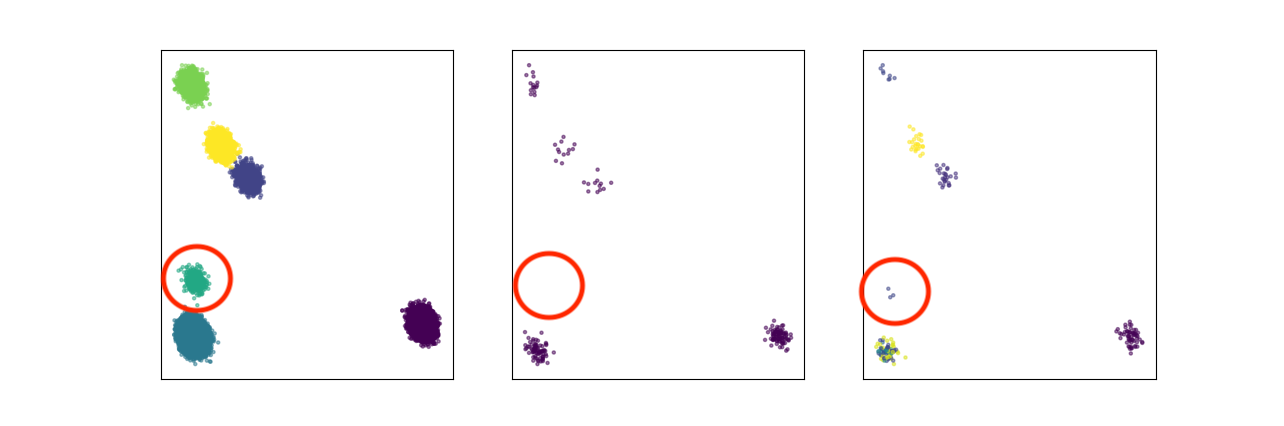
\includegraphics[width=.95\linewidth]{images/lightweight_breaks.png}
\caption{
The results of lightweight and fast-coreset constructions on a dataset of $n=100K$ points with clusters of varying size. Coresets have 200 points.
\emph{Left}: Original multivariate-Gaussian dataset. \emph{Middle}: Lightweight coresets fail to capture the cluster of $\sim$400 points.
\emph{Right}: The Fast-coreset construction runs in linear time but identifies all of the clusters.
}
\end{figure*}

\begin{figure}
    \centering
    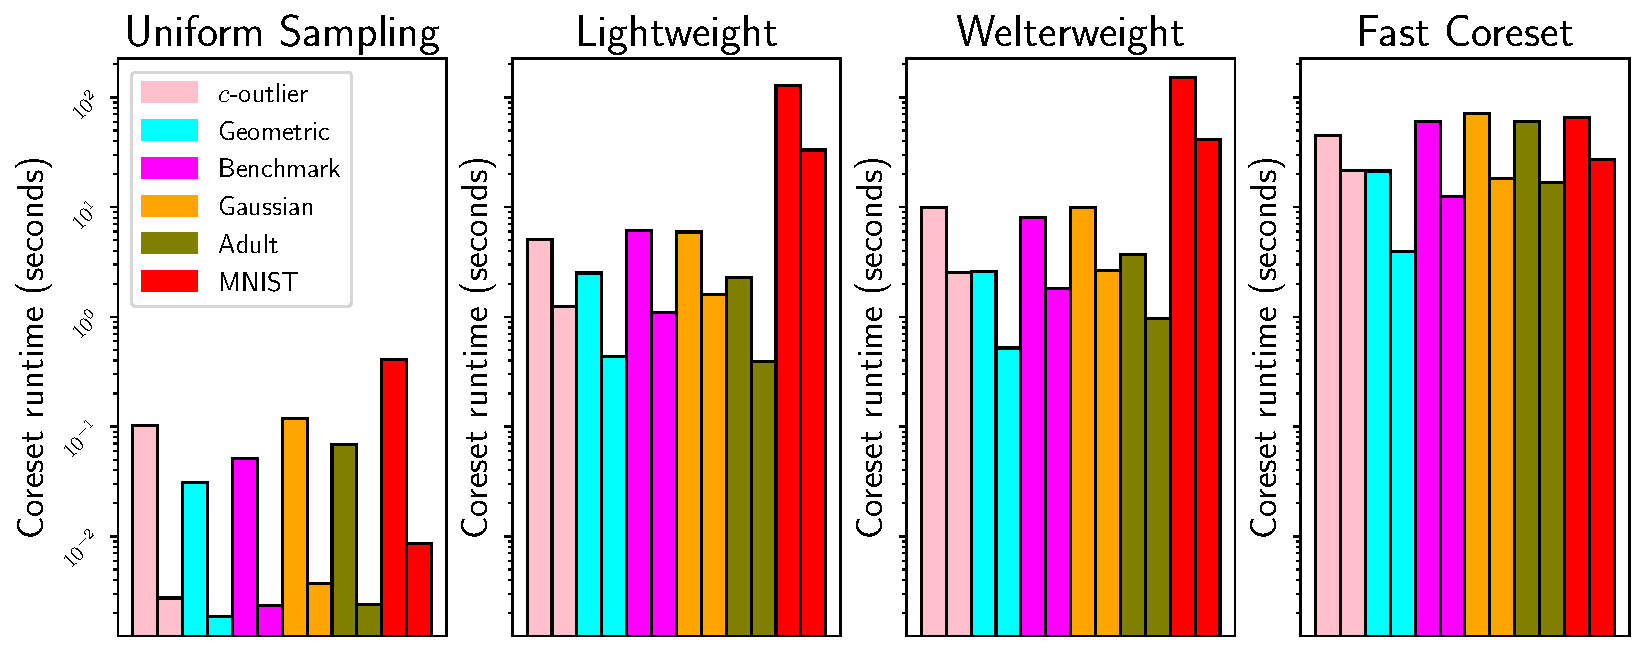
\includegraphics[width=.95\linewidth]{images/2/coreset_runtime-composition.pdf}
    \caption{Mean runtime over three runs in the streaming and non-streaming settings. Bars are [Streaming, Non-Streaming]; y-axis is log-scale.}
    \label{fig:coreset_size_on_sens_quality}
\end{figure}


\section{Data Parameters}
\label{app:data_params}
In all real and artificial datasets, we add random uniform noise $\eta$ with $0 \leq \eta_i \leq 0.001$ in each dimension in order to make all points unique.
Unless specifically varying these parameters, we default all algorithms in~\ref{ssec:algorithms} to $k=100$ for the Adult, MNIST, and artificial datasets and
$k=500$ for the Song, Cover Type, and Census datasets. Our default coreset size is then $m = 40k$. We refer to the coreset size scalar as the \emph{$m$-scalar}.
We only run the dimension-reduction step on the MNIST dataset, as the remaining datasets already have sufficiently low dimensionality.

\begin{table}[htbp]
    \centering
    \begin{tabular}{lrr}
        Dataset & Points & Dim \\
        \hline
        \emph{Adult} & 48\,842 & 14 \\
        \emph{MNIST} & 60\,000 & 784 \\
        \emph{Song} & 515\,345 & 90 \\
        \emph{Cover Type} & 581\,012 & 54 \\
        \emph{Census} & 2\,458\,285 & 68 \\
        \hline
        \vspace*{0.1cm}
    \end{tabular}
    \caption{Description of real world datasets}
    \label{tbl:datasets}
\end{table}

\begin{figure}
\centering
\begin{tabular}{lc}
    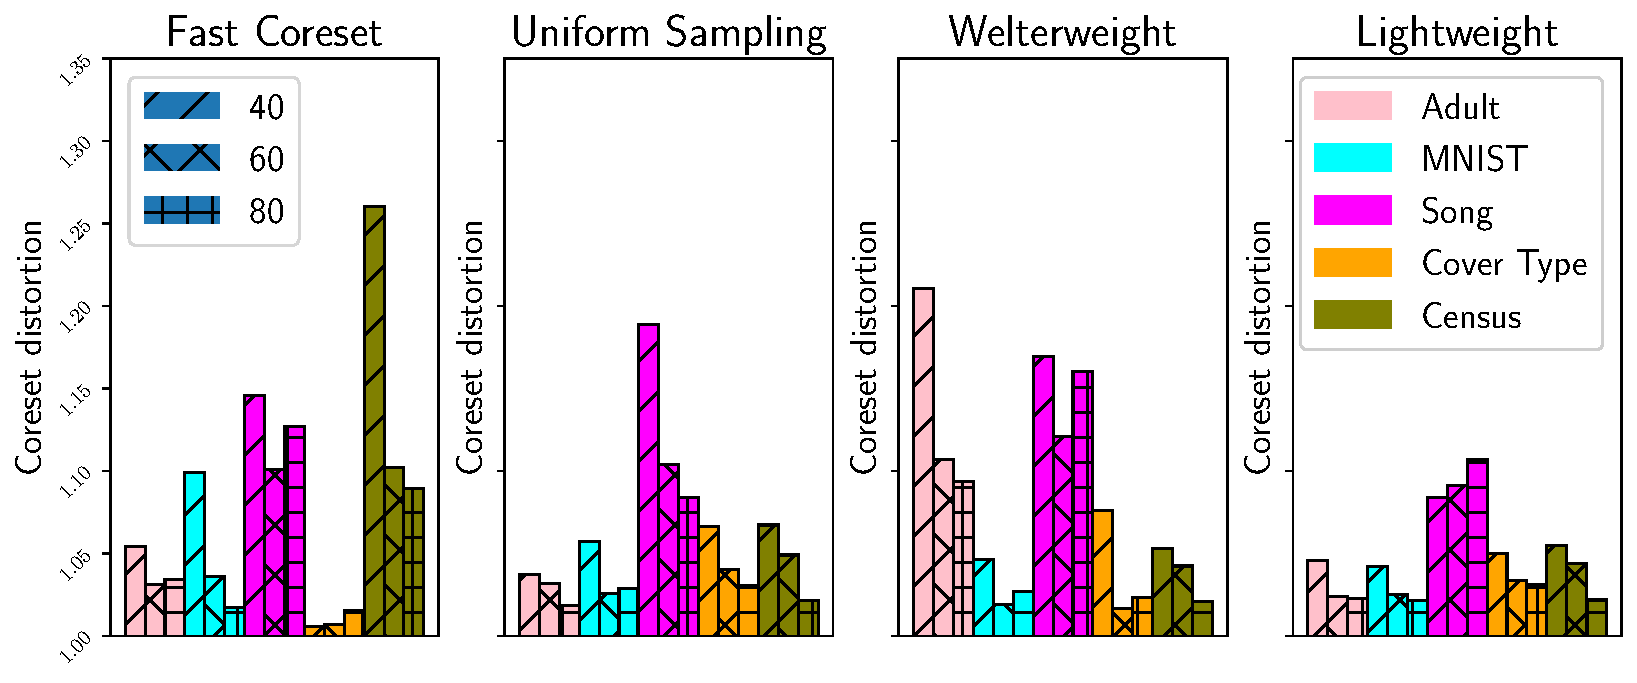
\includegraphics[width=\linewidth]{images/distortion_real_data} \\
    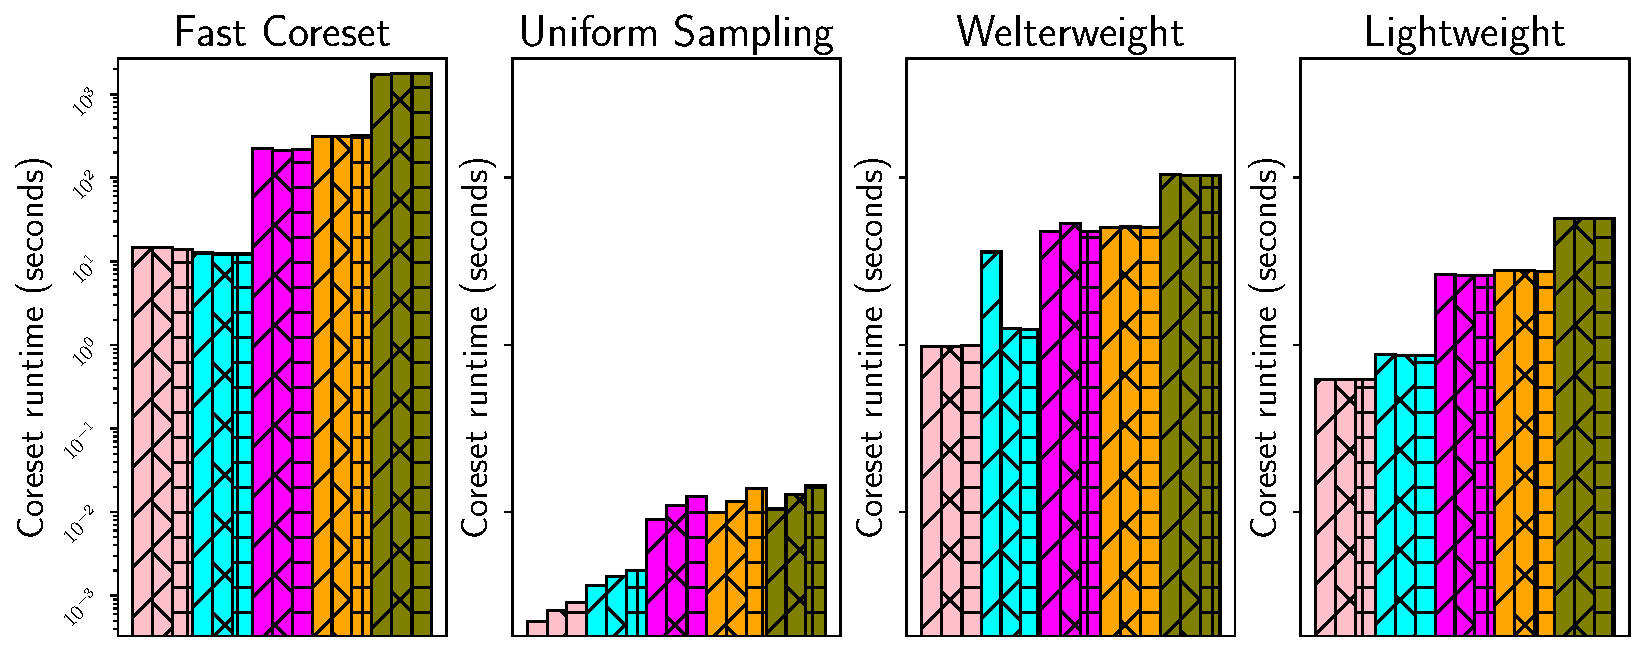
\includegraphics[width=\linewidth]{images/runtime_real_data}
\end{tabular}

\caption{\emph{Top}: The effect of the $m$-scalar on coreset distortion for real-world datasets. This is a visualization of the data in
Table~\ref{tbl:distortion}.  \emph{Bottom}: The effect of the $m$-scalar on the algorithm runtime for real-world datasets. All values are the mean over 5 runs.
The three bars represent samples of size $m=40k, 60k, 80k$.}

\label{fig:coreset_size_on_quality}
\end{figure}

